% Created by tikzDevice version 0.12.6 on 2025-02-12 13:10:31
% !TEX encoding = UTF-8 Unicode
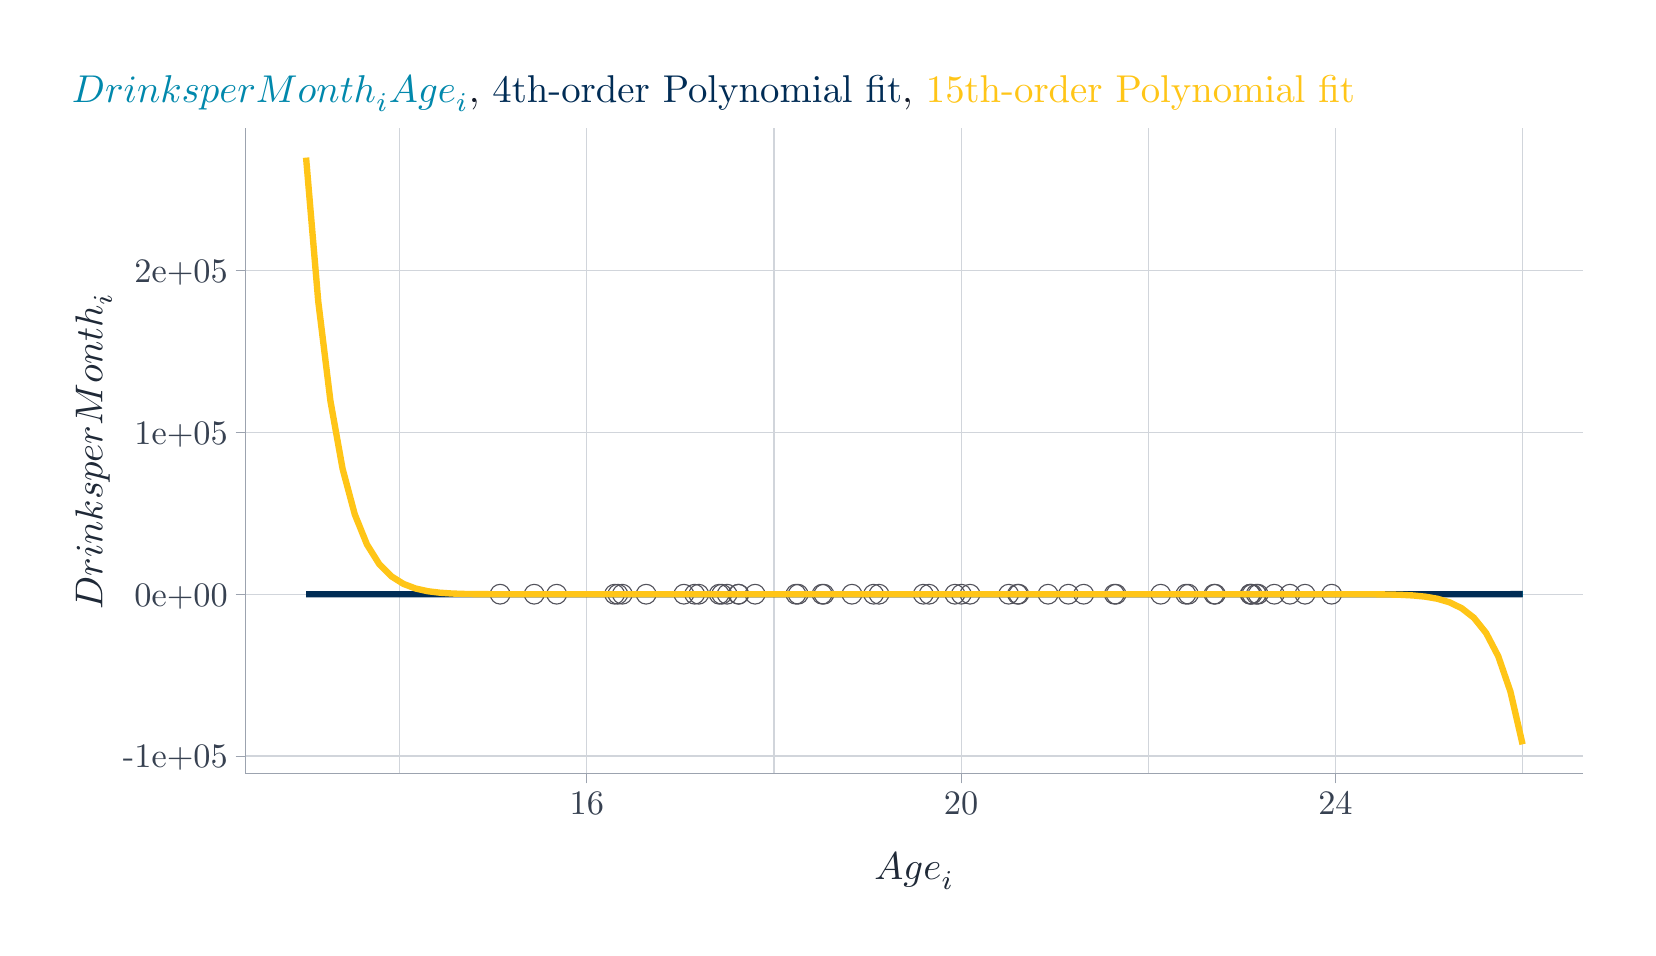
\begin{tikzpicture}[x=1pt,y=1pt]
\definecolor{fillColor}{RGB}{255,255,255}
\path[use as bounding box,fill=fillColor] (0,0) rectangle (578.16,325.21);
\begin{scope}
\path[clip] (  0.00,  0.00) rectangle (578.16,325.21);
\definecolor{drawColor}{RGB}{255,255,255}

\path[draw=drawColor,line width= 0.7pt,line join=round,line cap=round,fill=fillColor] (  0.00,  0.00) rectangle (578.16,325.21);
\end{scope}
\begin{scope}
\path[clip] ( 78.62, 55.65) rectangle (562.16,288.85);
\definecolor{drawColor}{RGB}{255,255,255}
\definecolor{fillColor}{RGB}{255,255,255}

\path[draw=drawColor,line width= 0.7pt,line join=round,line cap=round,fill=fillColor] ( 78.62, 55.65) rectangle (562.16,288.85);
\definecolor{drawColor}{RGB}{209,213,219}

\path[draw=drawColor,line width= 0.4pt,line join=round] (134.42, 55.65) --
	(134.42,288.85);

\path[draw=drawColor,line width= 0.4pt,line join=round] (269.67, 55.65) --
	(269.67,288.85);

\path[draw=drawColor,line width= 0.4pt,line join=round] (404.93, 55.65) --
	(404.93,288.85);

\path[draw=drawColor,line width= 0.4pt,line join=round] (540.18, 55.65) --
	(540.18,288.85);

\path[draw=drawColor,line width= 0.4pt,line join=round] ( 78.62, 62.01) --
	(562.16, 62.01);

\path[draw=drawColor,line width= 0.4pt,line join=round] ( 78.62,120.49) --
	(562.16,120.49);

\path[draw=drawColor,line width= 0.4pt,line join=round] ( 78.62,178.96) --
	(562.16,178.96);

\path[draw=drawColor,line width= 0.4pt,line join=round] ( 78.62,237.44) --
	(562.16,237.44);

\path[draw=drawColor,line width= 0.4pt,line join=round] (202.04, 55.65) --
	(202.04,288.85);

\path[draw=drawColor,line width= 0.4pt,line join=round] (337.30, 55.65) --
	(337.30,288.85);

\path[draw=drawColor,line width= 0.4pt,line join=round] (472.55, 55.65) --
	(472.55,288.85);
\definecolor{drawColor}{RGB}{82,82,91}

\path[draw=drawColor,line width= 0.4pt,line join=round,line cap=round] (256.80,120.49) circle (  3.57);

\path[draw=drawColor,line width= 0.4pt,line join=round,line cap=round] (250.80,120.49) circle (  3.57);

\path[draw=drawColor,line width= 0.4pt,line join=round,line cap=round] (191.15,120.49) circle (  3.57);

\path[draw=drawColor,line width= 0.4pt,line join=round,line cap=round] (241.00,120.49) circle (  3.57);

\path[draw=drawColor,line width= 0.4pt,line join=round,line cap=round] (183.03,120.49) circle (  3.57);

\path[draw=drawColor,line width= 0.4pt,line join=round,line cap=round] (337.38,120.49) circle (  3.57);

\path[draw=drawColor,line width= 0.4pt,line join=round,line cap=round] (256.96,120.49) circle (  3.57);

\path[draw=drawColor,line width= 0.4pt,line join=round,line cap=round] (278.42,120.49) circle (  3.57);

\path[draw=drawColor,line width= 0.4pt,line join=round,line cap=round] (357.66,120.49) circle (  3.57);

\path[draw=drawColor,line width= 0.4pt,line join=round,line cap=round] (307.62,120.49) circle (  3.57);

\path[draw=drawColor,line width= 0.4pt,line join=round,line cap=round] (442.41,120.49) circle (  3.57);

\path[draw=drawColor,line width= 0.4pt,line join=round,line cap=round] (419.44,120.49) circle (  3.57);

\path[draw=drawColor,line width= 0.4pt,line join=round,line cap=round] (277.59,120.49) circle (  3.57);

\path[draw=drawColor,line width= 0.4pt,line join=round,line cap=round] (409.42,120.49) circle (  3.57);

\path[draw=drawColor,line width= 0.4pt,line join=round,line cap=round] (212.08,120.49) circle (  3.57);

\path[draw=drawColor,line width= 0.4pt,line join=round,line cap=round] (262.86,120.49) circle (  3.57);

\path[draw=drawColor,line width= 0.4pt,line join=round,line cap=round] (252.74,120.49) circle (  3.57);

\path[draw=drawColor,line width= 0.4pt,line join=round,line cap=round] (213.26,120.49) circle (  3.57);

\path[draw=drawColor,line width= 0.4pt,line join=round,line cap=round] (287.05,120.49) circle (  3.57);

\path[draw=drawColor,line width= 0.4pt,line join=round,line cap=round] (441.86,120.49) circle (  3.57);

\path[draw=drawColor,line width= 0.4pt,line join=round,line cap=round] (392.66,120.49) circle (  3.57);

\path[draw=drawColor,line width= 0.4pt,line join=round,line cap=round] (305.66,120.49) circle (  3.57);

\path[draw=drawColor,line width= 0.4pt,line join=round,line cap=round] (287.71,120.49) circle (  3.57);

\path[draw=drawColor,line width= 0.4pt,line join=round,line cap=round] (418.51,120.49) circle (  3.57);

\path[draw=drawColor,line width= 0.4pt,line join=round,line cap=round] (444.61,120.49) circle (  3.57);

\path[draw=drawColor,line width= 0.4pt,line join=round,line cap=round] (323.63,120.49) circle (  3.57);

\path[draw=drawColor,line width= 0.4pt,line join=round,line cap=round] (223.48,120.49) circle (  3.57);

\path[draw=drawColor,line width= 0.4pt,line join=round,line cap=round] (441.73,120.49) circle (  3.57);

\path[draw=drawColor,line width= 0.4pt,line join=round,line cap=round] (297.85,120.49) circle (  3.57);

\path[draw=drawColor,line width= 0.4pt,line join=round,line cap=round] (443.94,120.49) circle (  3.57);

\path[draw=drawColor,line width= 0.4pt,line join=round,line cap=round] (471.18,120.49) circle (  3.57);

\path[draw=drawColor,line width= 0.4pt,line join=round,line cap=round] (456.11,120.49) circle (  3.57);

\path[draw=drawColor,line width= 0.4pt,line join=round,line cap=round] (358.13,120.49) circle (  3.57);

\path[draw=drawColor,line width= 0.4pt,line join=round,line cap=round] (393.28,120.49) circle (  3.57);

\path[draw=drawColor,line width= 0.4pt,line join=round,line cap=round] (428.67,120.49) circle (  3.57);

\path[draw=drawColor,line width= 0.4pt,line join=round,line cap=round] (368.71,120.49) circle (  3.57);

\path[draw=drawColor,line width= 0.4pt,line join=round,line cap=round] (249.87,120.49) circle (  3.57);

\path[draw=drawColor,line width= 0.4pt,line join=round,line cap=round] (340.51,120.49) circle (  3.57);

\path[draw=drawColor,line width= 0.4pt,line join=round,line cap=round] (461.56,120.49) circle (  3.57);

\path[draw=drawColor,line width= 0.4pt,line join=round,line cap=round] (325.72,120.49) circle (  3.57);

\path[draw=drawColor,line width= 0.4pt,line join=round,line cap=round] (242.50,120.49) circle (  3.57);

\path[draw=drawColor,line width= 0.4pt,line join=round,line cap=round] (450.46,120.49) circle (  3.57);

\path[draw=drawColor,line width= 0.4pt,line join=round,line cap=round] (354.48,120.49) circle (  3.57);

\path[draw=drawColor,line width= 0.4pt,line join=round,line cap=round] (429.15,120.49) circle (  3.57);

\path[draw=drawColor,line width= 0.4pt,line join=round,line cap=round] (237.11,120.49) circle (  3.57);

\path[draw=drawColor,line width= 0.4pt,line join=round,line cap=round] (214.88,120.49) circle (  3.57);

\path[draw=drawColor,line width= 0.4pt,line join=round,line cap=round] (376.05,120.49) circle (  3.57);

\path[draw=drawColor,line width= 0.4pt,line join=round,line cap=round] (381.58,120.49) circle (  3.57);

\path[draw=drawColor,line width= 0.4pt,line join=round,line cap=round] (170.72,120.49) circle (  3.57);

\path[draw=drawColor,line width= 0.4pt,line join=round,line cap=round] (335.05,120.49) circle (  3.57);
\definecolor{drawColor}{RGB}{1,136,172}

\path[draw=drawColor,line width= 2.3pt,line join=round] (100.60,120.49) --
	(105.00,120.49) --
	(109.40,120.49) --
	(113.79,120.49) --
	(118.19,120.49) --
	(122.58,120.49) --
	(126.98,120.49) --
	(131.37,120.49) --
	(135.77,120.49) --
	(140.17,120.49) --
	(144.56,120.49) --
	(148.96,120.49) --
	(153.35,120.49) --
	(157.75,120.49) --
	(162.14,120.49) --
	(166.54,120.49) --
	(170.94,120.49) --
	(175.33,120.49) --
	(179.73,120.49) --
	(184.12,120.49) --
	(188.52,120.49) --
	(192.91,120.49) --
	(197.31,120.49) --
	(201.71,120.49) --
	(206.10,120.49) --
	(210.50,120.49) --
	(214.89,120.49) --
	(219.29,120.49) --
	(223.69,120.49) --
	(228.08,120.49) --
	(232.48,120.49) --
	(236.87,120.49) --
	(241.27,120.49) --
	(245.66,120.49) --
	(250.06,120.49) --
	(254.46,120.49) --
	(258.85,120.49) --
	(263.25,120.49) --
	(267.64,120.49) --
	(272.04,120.49) --
	(276.43,120.49) --
	(280.83,120.49) --
	(285.23,120.49) --
	(289.62,120.49) --
	(294.02,120.49) --
	(298.41,120.49) --
	(302.81,120.49) --
	(307.21,120.49) --
	(311.60,120.49) --
	(316.00,120.49) --
	(320.39,120.49) --
	(324.79,120.49) --
	(329.18,120.49) --
	(333.58,120.49) --
	(337.98,120.49) --
	(342.37,120.49) --
	(346.77,120.49) --
	(351.16,120.49) --
	(355.56,120.49) --
	(359.95,120.49) --
	(364.35,120.49) --
	(368.75,120.49) --
	(373.14,120.49) --
	(377.54,120.49) --
	(381.93,120.49) --
	(386.33,120.49) --
	(390.72,120.49) --
	(395.12,120.49) --
	(399.52,120.49) --
	(403.91,120.49) --
	(408.31,120.49) --
	(412.70,120.49) --
	(417.10,120.49) --
	(421.50,120.49) --
	(425.89,120.49) --
	(430.29,120.49) --
	(434.68,120.49) --
	(439.08,120.49) --
	(443.47,120.49) --
	(447.87,120.49) --
	(452.27,120.49) --
	(456.66,120.49) --
	(461.06,120.49) --
	(465.45,120.49) --
	(469.85,120.49) --
	(474.24,120.49) --
	(478.64,120.49) --
	(483.04,120.49) --
	(487.43,120.49) --
	(491.83,120.49) --
	(496.22,120.49) --
	(500.62,120.49) --
	(505.01,120.49) --
	(509.41,120.49) --
	(513.81,120.49) --
	(518.20,120.49) --
	(522.60,120.49) --
	(526.99,120.49) --
	(531.39,120.49) --
	(535.79,120.49) --
	(540.18,120.49);
\definecolor{drawColor}{RGB}{0,44,85}

\path[draw=drawColor,line width= 2.3pt,line join=round] (100.60,120.49) --
	(105.00,120.49) --
	(109.40,120.49) --
	(113.79,120.49) --
	(118.19,120.49) --
	(122.58,120.49) --
	(126.98,120.49) --
	(131.37,120.49) --
	(135.77,120.49) --
	(140.17,120.49) --
	(144.56,120.49) --
	(148.96,120.49) --
	(153.35,120.49) --
	(157.75,120.49) --
	(162.14,120.49) --
	(166.54,120.49) --
	(170.94,120.49) --
	(175.33,120.49) --
	(179.73,120.49) --
	(184.12,120.49) --
	(188.52,120.49) --
	(192.91,120.49) --
	(197.31,120.49) --
	(201.71,120.49) --
	(206.10,120.49) --
	(210.50,120.49) --
	(214.89,120.49) --
	(219.29,120.49) --
	(223.69,120.49) --
	(228.08,120.49) --
	(232.48,120.49) --
	(236.87,120.49) --
	(241.27,120.49) --
	(245.66,120.49) --
	(250.06,120.49) --
	(254.46,120.49) --
	(258.85,120.49) --
	(263.25,120.49) --
	(267.64,120.49) --
	(272.04,120.49) --
	(276.43,120.49) --
	(280.83,120.49) --
	(285.23,120.49) --
	(289.62,120.49) --
	(294.02,120.49) --
	(298.41,120.49) --
	(302.81,120.49) --
	(307.21,120.49) --
	(311.60,120.49) --
	(316.00,120.49) --
	(320.39,120.49) --
	(324.79,120.49) --
	(329.18,120.49) --
	(333.58,120.49) --
	(337.98,120.49) --
	(342.37,120.49) --
	(346.77,120.49) --
	(351.16,120.49) --
	(355.56,120.49) --
	(359.95,120.49) --
	(364.35,120.49) --
	(368.75,120.49) --
	(373.14,120.49) --
	(377.54,120.49) --
	(381.93,120.49) --
	(386.33,120.49) --
	(390.72,120.49) --
	(395.12,120.49) --
	(399.52,120.49) --
	(403.91,120.49) --
	(408.31,120.49) --
	(412.70,120.49) --
	(417.10,120.49) --
	(421.50,120.49) --
	(425.89,120.49) --
	(430.29,120.49) --
	(434.68,120.49) --
	(439.08,120.49) --
	(443.47,120.49) --
	(447.87,120.49) --
	(452.27,120.49) --
	(456.66,120.49) --
	(461.06,120.49) --
	(465.45,120.49) --
	(469.85,120.49) --
	(474.24,120.49) --
	(478.64,120.49) --
	(483.04,120.49) --
	(487.43,120.49) --
	(491.83,120.49) --
	(496.22,120.49) --
	(500.62,120.49) --
	(505.01,120.49) --
	(509.41,120.49) --
	(513.81,120.49) --
	(518.20,120.49) --
	(522.60,120.49) --
	(526.99,120.49) --
	(531.39,120.49) --
	(535.79,120.50) --
	(540.18,120.50);
\definecolor{drawColor}{RGB}{255,197,23}

\path[draw=drawColor,line width= 2.3pt,line join=round] (100.60,278.25) --
	(105.00,226.27) --
	(109.40,190.33) --
	(113.79,165.83) --
	(118.19,149.37) --
	(122.58,138.50) --
	(126.98,131.46) --
	(131.37,126.99) --
	(135.77,124.22) --
	(140.17,122.55) --
	(144.56,121.57) --
	(148.96,121.03) --
	(153.35,120.74) --
	(157.75,120.59) --
	(162.14,120.52) --
	(166.54,120.50) --
	(170.94,120.49) --
	(175.33,120.49) --
	(179.73,120.49) --
	(184.12,120.49) --
	(188.52,120.49) --
	(192.91,120.49) --
	(197.31,120.49) --
	(201.71,120.49) --
	(206.10,120.49) --
	(210.50,120.49) --
	(214.89,120.49) --
	(219.29,120.49) --
	(223.69,120.49) --
	(228.08,120.49) --
	(232.48,120.49) --
	(236.87,120.49) --
	(241.27,120.49) --
	(245.66,120.49) --
	(250.06,120.49) --
	(254.46,120.49) --
	(258.85,120.49) --
	(263.25,120.49) --
	(267.64,120.49) --
	(272.04,120.49) --
	(276.43,120.49) --
	(280.83,120.49) --
	(285.23,120.49) --
	(289.62,120.49) --
	(294.02,120.49) --
	(298.41,120.49) --
	(302.81,120.49) --
	(307.21,120.49) --
	(311.60,120.49) --
	(316.00,120.49) --
	(320.39,120.49) --
	(324.79,120.49) --
	(329.18,120.49) --
	(333.58,120.49) --
	(337.98,120.49) --
	(342.37,120.49) --
	(346.77,120.49) --
	(351.16,120.49) --
	(355.56,120.49) --
	(359.95,120.49) --
	(364.35,120.49) --
	(368.75,120.49) --
	(373.14,120.49) --
	(377.54,120.49) --
	(381.93,120.49) --
	(386.33,120.49) --
	(390.72,120.49) --
	(395.12,120.49) --
	(399.52,120.49) --
	(403.91,120.49) --
	(408.31,120.49) --
	(412.70,120.49) --
	(417.10,120.49) --
	(421.50,120.49) --
	(425.89,120.49) --
	(430.29,120.49) --
	(434.68,120.49) --
	(439.08,120.49) --
	(443.47,120.49) --
	(447.87,120.49) --
	(452.27,120.49) --
	(456.66,120.49) --
	(461.06,120.49) --
	(465.45,120.49) --
	(469.85,120.49) --
	(474.24,120.49) --
	(478.64,120.49) --
	(483.04,120.48) --
	(487.43,120.45) --
	(491.83,120.39) --
	(496.22,120.27) --
	(500.62,120.04) --
	(505.01,119.61) --
	(509.41,118.85) --
	(513.81,117.55) --
	(518.20,115.41) --
	(522.60,111.95) --
	(526.99,106.49) --
	(531.39, 98.07) --
	(535.79, 85.30) --
	(540.18, 66.25);
\end{scope}
\begin{scope}
\path[clip] (  0.00,  0.00) rectangle (578.16,325.21);
\definecolor{drawColor}{RGB}{156,163,175}

\path[draw=drawColor,line width= 0.3pt,line join=round] ( 78.62, 55.65) --
	( 78.62,288.85);
\end{scope}
\begin{scope}
\path[clip] (  0.00,  0.00) rectangle (578.16,325.21);
\definecolor{drawColor}{RGB}{55,65,81}

\node[text=drawColor,anchor=base east,inner sep=0pt, outer sep=0pt, scale=  1.24] at ( 72.32, 57.73) {-1e+05};

\node[text=drawColor,anchor=base east,inner sep=0pt, outer sep=0pt, scale=  1.24] at ( 72.32,116.20) {0e+00};

\node[text=drawColor,anchor=base east,inner sep=0pt, outer sep=0pt, scale=  1.24] at ( 72.32,174.68) {1e+05};

\node[text=drawColor,anchor=base east,inner sep=0pt, outer sep=0pt, scale=  1.24] at ( 72.32,233.16) {2e+05};
\end{scope}
\begin{scope}
\path[clip] (  0.00,  0.00) rectangle (578.16,325.21);
\definecolor{drawColor}{RGB}{156,163,175}

\path[draw=drawColor,line width= 0.3pt,line join=round] ( 75.12, 62.01) --
	( 78.62, 62.01);

\path[draw=drawColor,line width= 0.3pt,line join=round] ( 75.12,120.49) --
	( 78.62,120.49);

\path[draw=drawColor,line width= 0.3pt,line join=round] ( 75.12,178.96) --
	( 78.62,178.96);

\path[draw=drawColor,line width= 0.3pt,line join=round] ( 75.12,237.44) --
	( 78.62,237.44);
\end{scope}
\begin{scope}
\path[clip] (  0.00,  0.00) rectangle (578.16,325.21);
\definecolor{drawColor}{RGB}{156,163,175}

\path[draw=drawColor,line width= 0.3pt,line join=round] ( 78.62, 55.65) --
	(562.16, 55.65);
\end{scope}
\begin{scope}
\path[clip] (  0.00,  0.00) rectangle (578.16,325.21);
\definecolor{drawColor}{RGB}{156,163,175}

\path[draw=drawColor,line width= 0.3pt,line join=round] (202.04, 52.15) --
	(202.04, 55.65);

\path[draw=drawColor,line width= 0.3pt,line join=round] (337.30, 52.15) --
	(337.30, 55.65);

\path[draw=drawColor,line width= 0.3pt,line join=round] (472.55, 52.15) --
	(472.55, 55.65);
\end{scope}
\begin{scope}
\path[clip] (  0.00,  0.00) rectangle (578.16,325.21);
\definecolor{drawColor}{RGB}{55,65,81}

\node[text=drawColor,anchor=base,inner sep=0pt, outer sep=0pt, scale=  1.24] at (202.04, 40.78) {16};

\node[text=drawColor,anchor=base,inner sep=0pt, outer sep=0pt, scale=  1.24] at (337.30, 40.78) {20};

\node[text=drawColor,anchor=base,inner sep=0pt, outer sep=0pt, scale=  1.24] at (472.55, 40.78) {24};
\end{scope}
\begin{scope}
\path[clip] (  0.00,  0.00) rectangle (578.16,325.21);
\definecolor{drawColor}{RGB}{31,41,55}

\node[text=drawColor,anchor=base,inner sep=0pt, outer sep=0pt, scale=  1.40] at (320.39, 17.36) {$\text{Age}_i$};
\end{scope}
\begin{scope}
\path[clip] (  0.00,  0.00) rectangle (578.16,325.21);
\definecolor{drawColor}{RGB}{31,41,55}

\node[text=drawColor,rotate= 90.00,anchor=base,inner sep=0pt, outer sep=0pt, scale=  1.40] at ( 27.00,172.25) {$\text{Drinks per Month}_i$};
\end{scope}
\begin{scope}
\path[clip] (  0.00,  0.00) rectangle (578.16,325.21);
\definecolor{drawColor}{RGB}{17,24,39}

\node[text=drawColor,anchor=base west,inner sep=0pt, outer sep=0pt, scale=  1.40] at ( 16.00,298.21) {{\color[HTML]{0188AC} $\expec{\text{Drinks per Month}_i}{\text{Age}_i}$}, {\color[HTML]{002C55} 4th-order Polynomial fit}, {\color[HTML]{ffc517} 15th-order Polynomial fit}};
\end{scope}
\end{tikzpicture}
